\chapter{Background}
% SE PÅ SamuelsenS MASTEROPPGAVE FOR INSPIRASJON (TROR HAN CLUSTERA OG KLASSIFISERTE HOVEDKONSEPTENE HAN BYGDE PÅ).

\gjor{Skriv opp bulletpoints fra mulige inspirasjoner og referanser her. "Write a few lines summarising relevant articles one comes across (which one is likely to refer to in the final report)" - Jims master-skrivingsdokument)}

\lab{Fra Essay-kommentarer} {
	\inkl {
		Often times, scientists have drawn inspiration from various scientific fields -- particularly different fields from ones own -- into their own field, for various reasons. Indeed, the translated concepts (from the one domain to the other) will most likely be accompanied with brand new ways to think about ones own domain, as well as other domains again interacting with it (hence having a real opportunity to start a "domino"-like chain-reaction of new ways to think about things emerging). These new ways to think about things (often in ones own domain) -- apart from being interesting and intriguing -- might be useful, both for ones own field but also for other fields again (especially if thinking long term). For example in the Multi-Agent Systems (MAS) field, it has been a common practice to study complex biological systems in nature, in order to translate these mechanisms into the technology- and engineering-domain (be it the \textit{Ant Colony(?)}, or \textit{Beeclust(?)}). Such bio-inspired algorithms have been -- \textit{and still are(?)} -- some of the most widely used optimization algorithms throughout history.
	}
	
	\inkl {
		(Fra Essay om 'path planning', 'EA's og 'multi-objective optimization'. Definitivt ikke kopier, men skriv om isåfall): "This essay attempts to give an overview over the fields of path-planning, evolutionary algorithms and multi-objective optimization, including pointers to recent work in these fields, especially where they intersect. In tradition with other literature relating to evolutionary algorithms, algorithms which are not population-based or otherwise based on principles similar to evolutionary algorithms are called ’classical’ to separate them from evolutionary variants."
	}
}

\tcol[gray]{\section{Nymoen et al. sin Firefly-Synkronisering:}}
	\inkl{
		\nl Nymoen et al. \cite{nymoen_synch} showed how one can, by endowing musical agents with self-awareness capabilities, achieve \textit{harmonic synchrony} of phases and frequencies in pulse-coupled oscillators.
		
		\sep
		
		% Recall of talk with Sigmund at the kitchen in M9
		% Recall av det jeg forklarte til Sigmund:
\lab{Sigmund Kjøkken-Recall}{
	\besk{Kanskje denne seksjonen blir gjort overflødig av en god forklaring på Oscillatorer og synkronisering av Oscillatorer i 'Background'-kapittelet, og en god forklaring av akkurat hvordan dette oppnås i 'Implementation'-kapittelet?}

	\gjor{Demonstrer/Illustrer poenget bak fingrene og tidsaksen på bordet (ish det som er i figuren under for fase), og så det samme for frekvens-justering med f.eks. halve—eller noe annet—som start-frekvens; og at de da ender i \textit{harmonisk synkroni}}

	\begin{figure}[h!]
		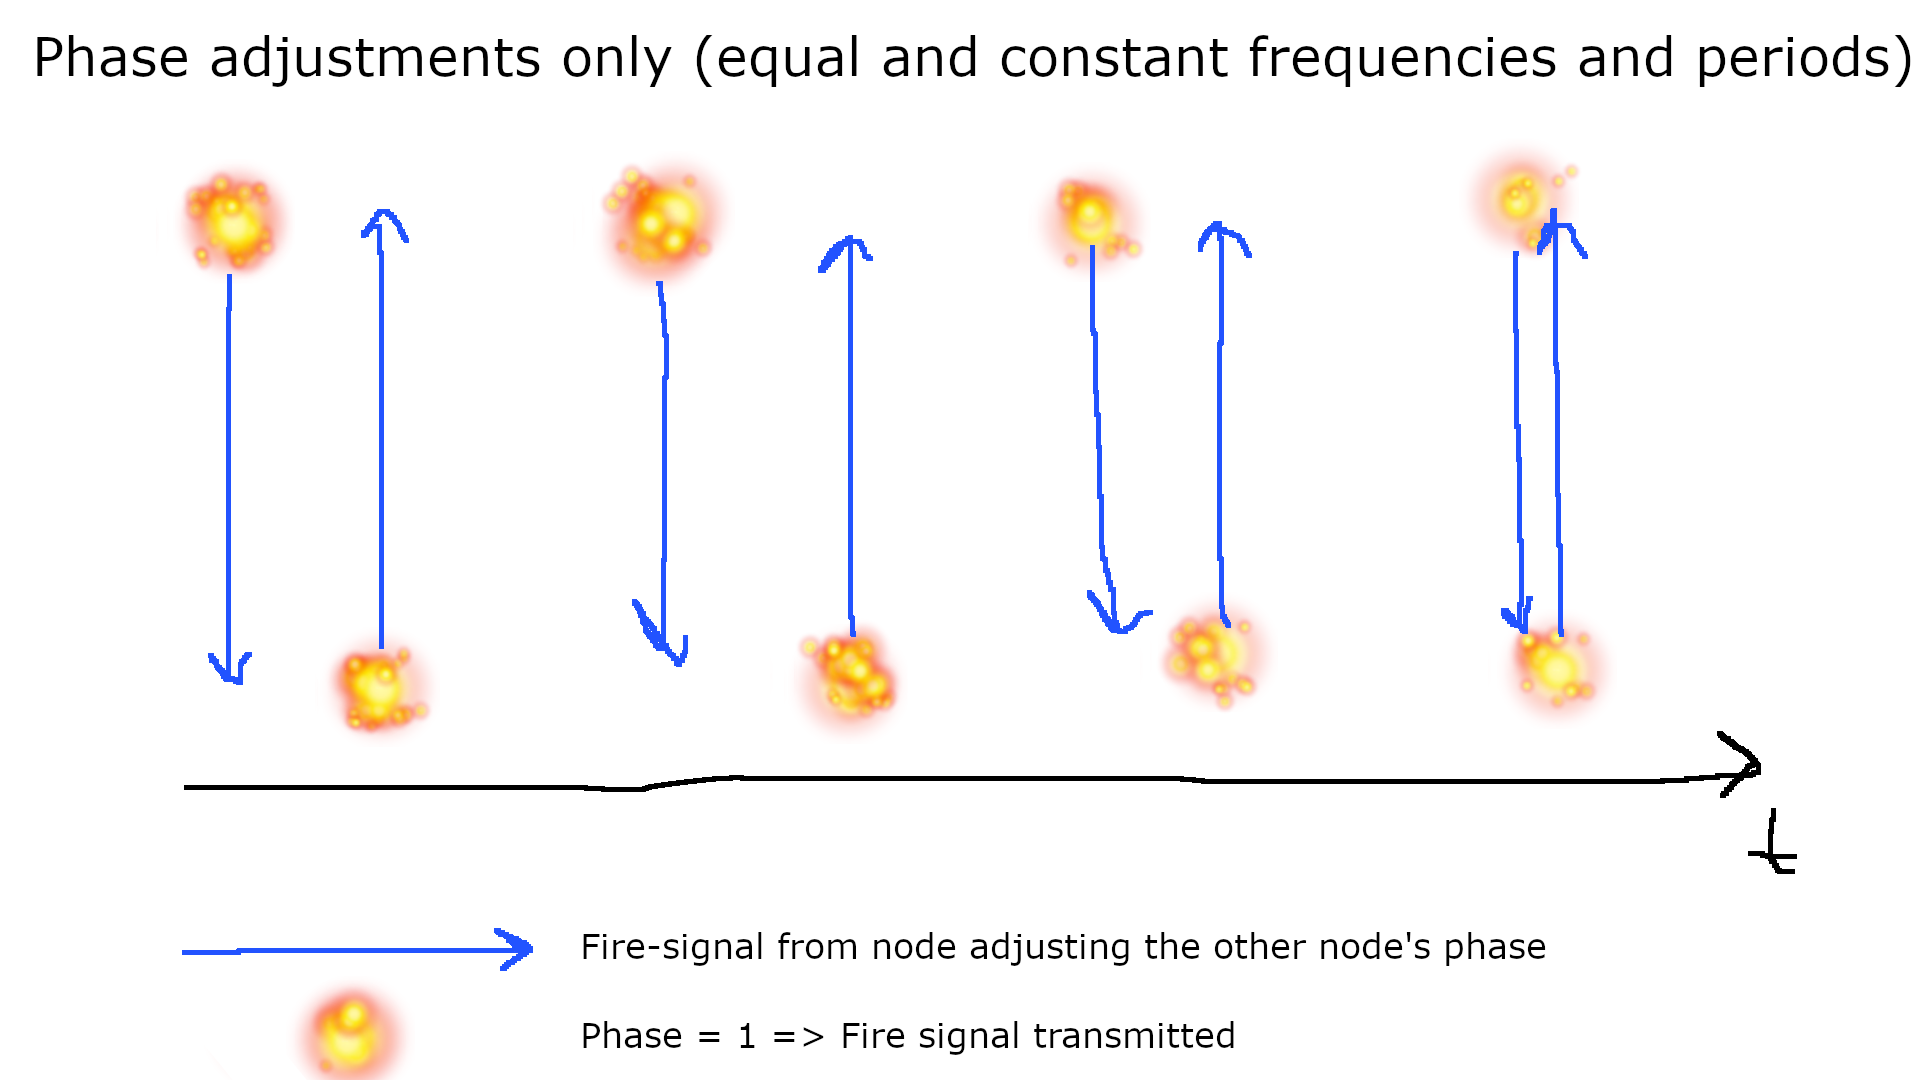
\includegraphics[width=0.90\textwidth]{Assets/Figures/phase_adjustments.png}
		\caption{Fase-justering (som om man skulle tappet med fingrene på et bord)}
	\end{figure}
}
		
		\sep
		
		% (Ish) Recall of talk with Kjersti at home in the livingroom (when she came with Lucky)
		\lab{Tante-Kjersti-inspirert {\normalsize (ish Stue-Recall)}}{
	The diverse and complex phenomena of nature have for long served as exciting inspirations to human engineering and research (cite ant colonies, boids \& swarms, beeclust e.g.). One such phenomena studied and attempted modelled is the synchronous firing of fireflies in the rainforests.
	\nl

	\gjor{Insert illustration/picture of synchronizing/synchronized fireflies firing in a dark forest here}

	This has inspired scientists like Mirollo \& Strogatz \cite{}, and in later time Kristian Nymoen, Kyrre Glette et al. \cite{nymoen_synch}, to attempt to model and "etterlikne" this natural phenomenon in human-engineered systems. This work ties into the work on synchronizing oscillators \powof{\cite{,,}} which has been subject to study for some time now. What separates Mirollo \& Strogatz and K. Nymoen's approach from these previous ones, is that here the oscillators are \tit{pulse-coupled}, as opposed to the more normal and constraining \tit{phase-coupled} (\powof{explain}).
	Each modelled "firefly", or firing node, is here implemented and considered as an oscillator, characterized by its phase and frequency. \inkl{Kinda, the job is to align sinusoidal waves, either by shifting an agent's phase "up", or "down".}
	
	\inkl{No training of any neural networks or any model-data was needed to achieve synchrony in this case — and so far no machine learning is used — but instead we see an emergent \tit{harmonic synchrony} in a collective, by endowing fairly simple agents with not too complicated update-functions. This is well known in the Multi-Agent Systems \& Swarm Robotics literature \powof{\cite{,,}}.}
}
	}

\section{Oscillators and Oscillator-Synchronization}

	\besk{Beskrive dette så godt at jeg kan snakke fritt om oscillatorers \textbf{faser} og \textbf{frekvenser} senere (i Implementation f.eks.), spesielt i tilfelle noen ikke har vært borti det før, eller tatt et Signalbehandlings-kurs}
	
	\gjor{Skill på Pulse-coupled Oscillators, og Phase-coupled Oscillators}
	